\documentclass[12pt]{article}
\usepackage[utf8]{inputenc}
\usepackage[greek,english]{babel}
\usepackage{alphabeta}
\usepackage{fancyhdr}
\usepackage{listings}
\usepackage{mathtools}
\usepackage{xcolor}
\usepackage{float}
\usepackage{siunitx}
\usepackage[margin=0.5in]{geometry}
\usepackage[backend=bibtex]{biblatex}

\title{Εργαστήριο Μικροηλεκτρονικής -- Εργασία 2}
\author{Χρήστος Μαργιώλης -- 19390133}
\date{Απρίλιος 2022}

\begin{document}

\begin{titlepage}
        \maketitle
        \begin{figure}[t!]
        \begin{center}
        
\includegraphics[scale=0.3]{./res/uniwalogo.png} \\
        \Large
        \textbf{Πανεπιστήμιο Δυτικής Αττικής} \\
        \large
        Τμήμα Μηχανικών Πληροφορικής και Ηλεκτρονικών Υπολογιστών
        \end{center}
        \end{figure}
\end{titlepage}

\renewcommand{\contentsname}{Περιεχόμενα}
\tableofcontents
\pagebreak

\section{Θεωρητικό μέρος}

Ο μη-αναστρέφων τελεστικός ενισχυτής είναι μία από τις διάφορες συνδεσμολογίες
τελεστικών ενισχυτών που υπάρχουν. Οι κύριες διαφορές του με τον αναστρέφοντα
ενισχυτή, είναι ότι, ο μη-αναστρέφων ενισχυτής παρουσιάζει πολύ μεγαλή
αντίσταση εισόδου, έχει υποχρεωτικά κέρδος μεγαλύτερο του 1, και το σήμα εξόδου
είναι σε φάση με το σήμα εισόδου.

Επιπλέον, ο μη-αναστρέφων ενισχυτής, έχει πολύ παρόμοια συνδεσμολογία με τον
buffer, με την διαφορά ότι ο buffer δεν περιέχει αντιστάσεις.

\section{Υλοποίηση της εργασίας}

Για την υλοποίηση της εργασίας χρησιμοποιήθηκαν τα παρακάτω εργαλεία:
\begin{itemize}
	\item Tina-TI για την συνδεσμολογία και τις μετρήσεις του κυκλώματος.
	\item Tinkercad για την υλοποίηση του κυκλώματος σε breadboard.
	\item \LaTeX για την συγγραφή της εργασίας.
\end{itemize}

\section{Συνδεσμολόγηση κυκλώματος}

\begin{itemize}
	\item Συνδεσμολογήστε το παρακάτω κύκλωμα με
		$R_1 = R_2 = \SI{10}{\kilo\ohm}$ και
		$V_1 = \SI{15}{\volt}$,
		$V_2 = \SI{-15}{\volt}$.
\end{itemize}

\begin{figure}[H]
	\centering
	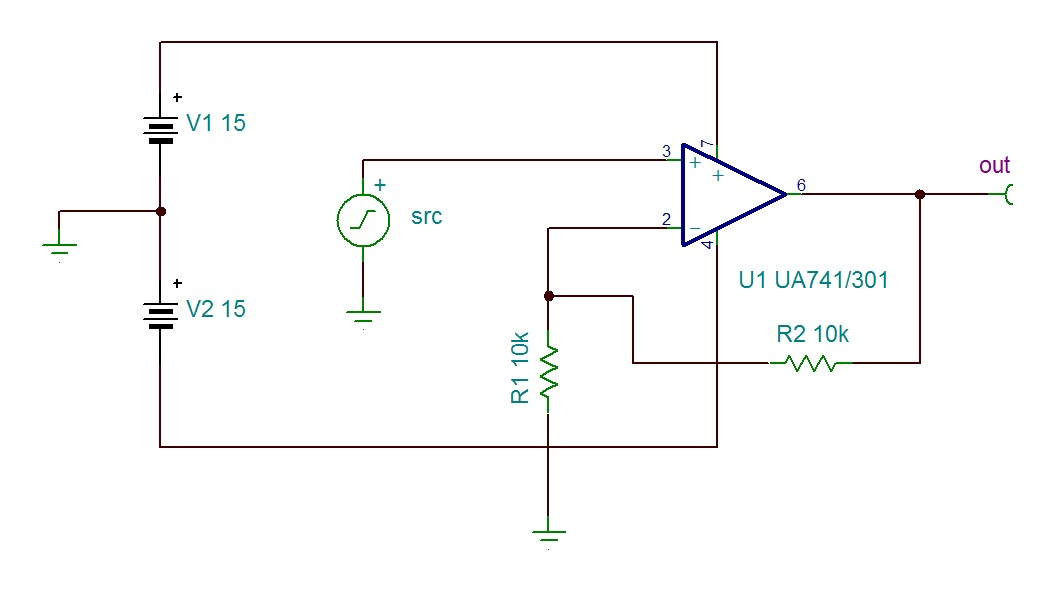
\includegraphics[width=\linewidth]{./res/schem.jpg}
	\caption{Μη-αναστρέφων τελεστικός ενισχυτής}
\end{figure}

\section{Εφαρμογή σήματος}

\begin{itemize}
	\item Εφαρμόστε ημιτονικό σήμα $\SI{1}{\kilo\hertz}/1V_{pp}$ στην είσοδο.
	\begin{itemize}
		\item Αναπαραστήσετε σε γράφημα την έξοδο του κυκλώματος ως
			προς την είσοδο.
		\item Υπολογίστε το θεωρητικό και πρακτικό κέρδος του ενισχυτή,
			στη συνέχεια συγκρίνατε τα δύο κέρδη. Υπάρχουν
			διαφορές; Πού οφείλονται;
		\item Μετρήστε την διαφορά φάσης που παρατηρείται μεταξύ
			εισόδου και εξόδου.
	\end{itemize}
\end{itemize}

\subsection{Γράφημα εξόδου ως προς είσοδο}

Το σήμα εξόδου είναι ενισχυμένο, και βρίσκεται σε φάση με το σήμα εισόδου.

\begin{figure}[H]
	\centering
	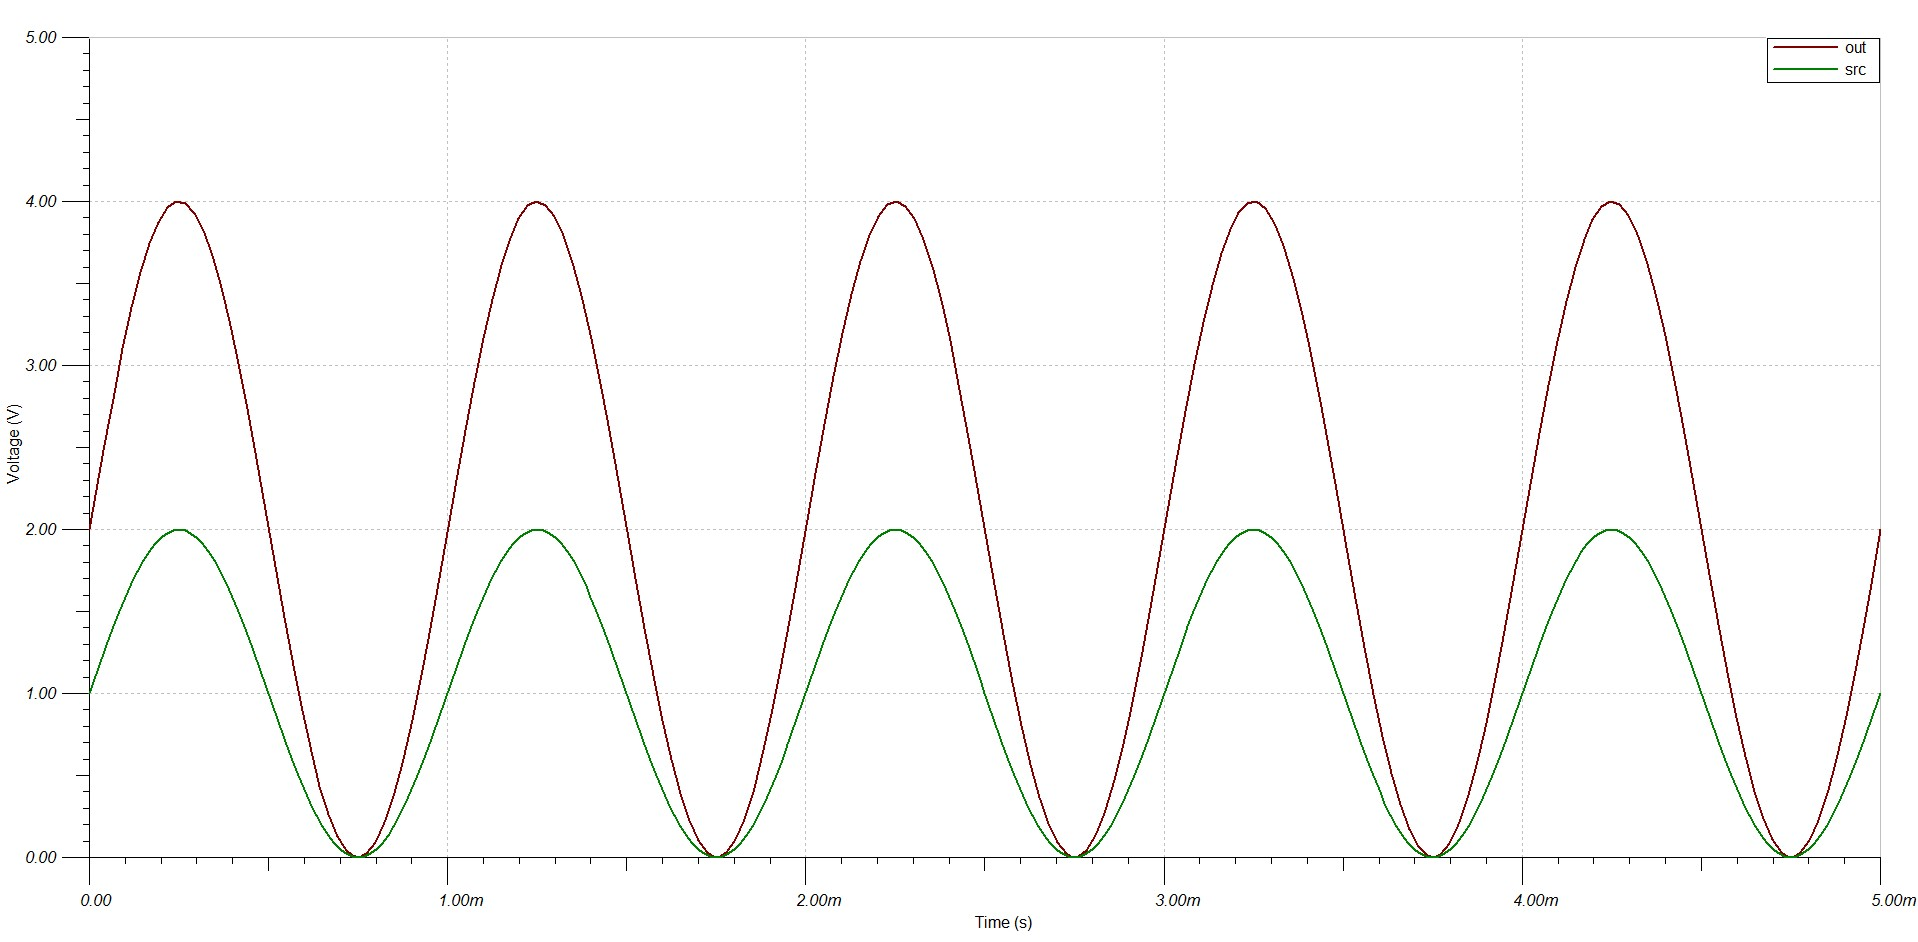
\includegraphics[width=\linewidth]{./res/out1.jpg}
	\caption{Καμπύλες στο ίδιο γράφημα}
\end{figure}

\begin{figure}[H]
	\centering
	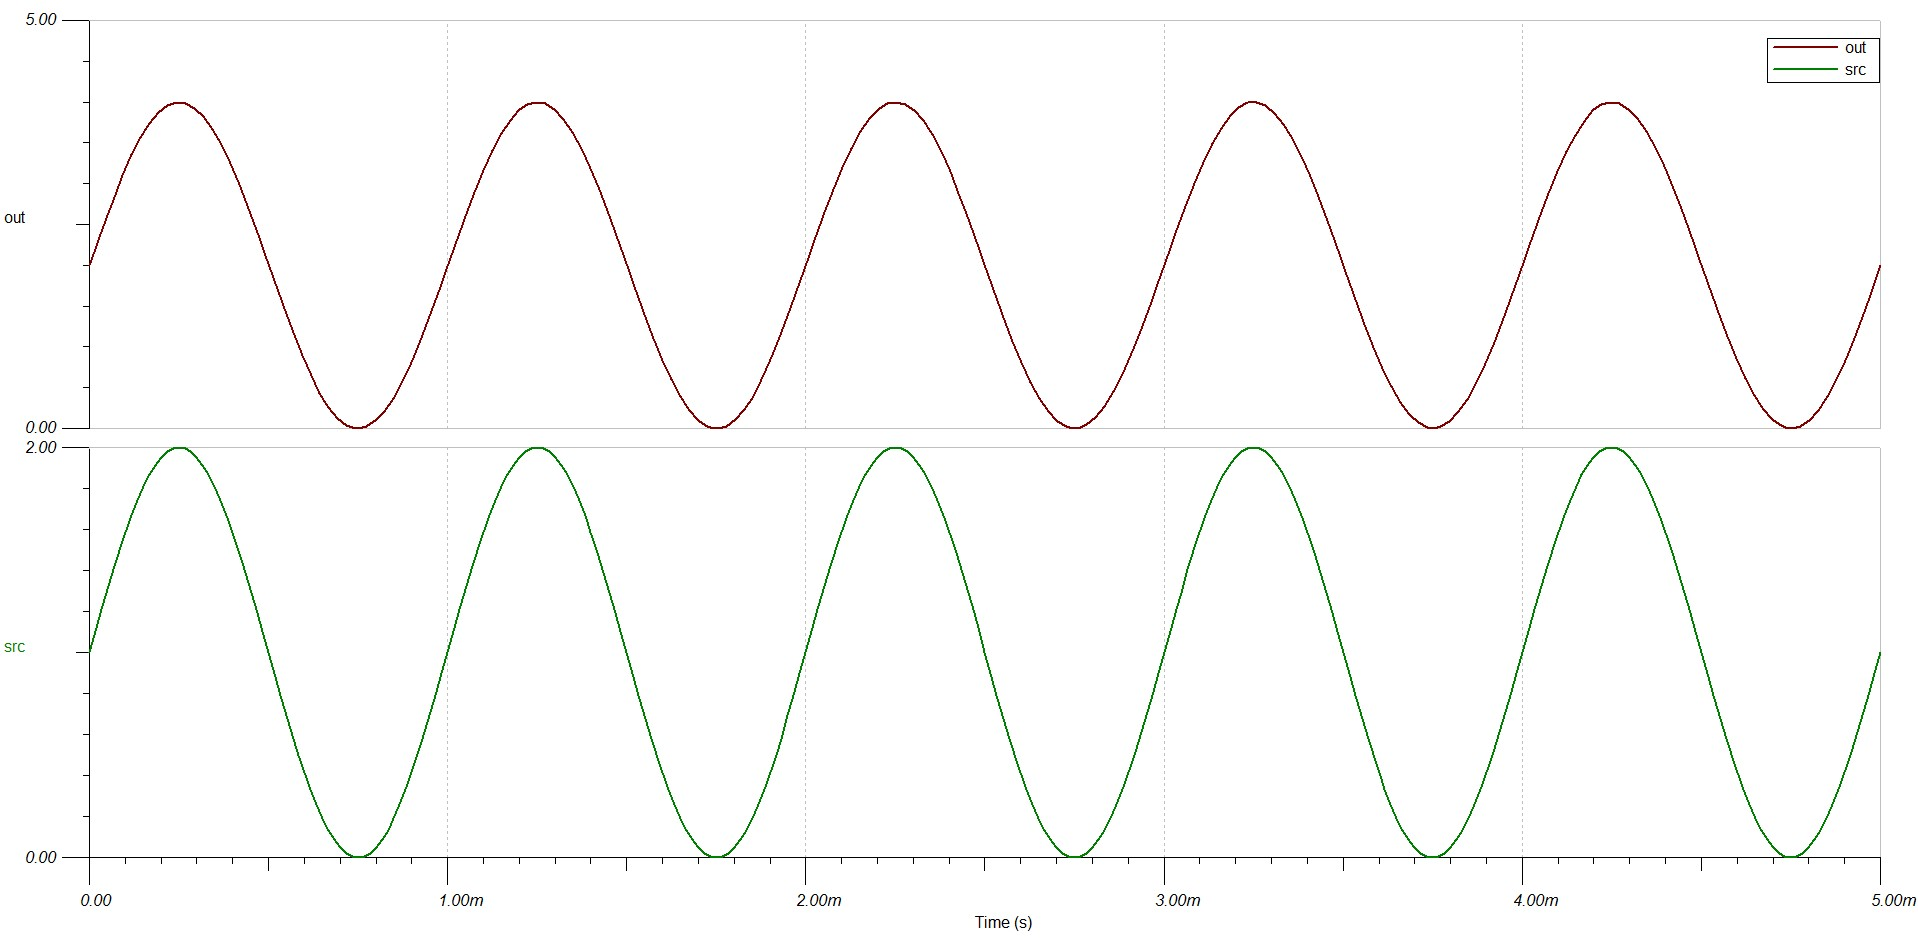
\includegraphics[width=\linewidth]{./res/out2.jpg}
	\caption{Καμπύλες σε ξεχωριστό γράφημα}
\end{figure}

\subsection{Θεωρητικό και πρακτικό κέρδος}

Το θεωρητικό κέρδος του μη-αναστρέφοντα τελεστικού ενισχυτή υπολογίζεται από
τον τύπο:
\[A_v = \frac{V_{out}}{V_{in}} = 1 + \frac{R_2}{R_1}\]
Οπότε, αντικαθιστώντας τις τιμές των αντιστάσεων, έχουμε ότι:
\[
	A_v = 1 + \frac{R_2}{R_1} \Rightarrow
	A_v = 1 + \frac{\SI{10}{\kilo\ohm}}{\SI{10}{\kilo\ohm}} \Rightarrow
	A_v = 1 + 1 \Rightarrow
	A_v = 2
\]
Μετατρέπουμε το γραμμικό κέρδος σε dB:
\[
	A_v(\SI{}{\decibel}) = 20\log_{10}\lvert A_v \lvert \Rightarrow
	A_v(\SI{}{\decibel}) = 20\log_{10} 2 \Rightarrow
	A_v(\SI{}{\decibel}) = \SI{6.02}{\decibel}
\]

Μελετώντας την μέτρηση του πρακτικού κέρδους στις παρακάτω εικόνες, παρατηρύμε
ότι οι υπολογισμοί συμπίπτουν. Επίσης, παρατηρούμε ότι μετά από μία
συγκεκριμένη συχνότητα, το κέρδος αρχίζει και πέφτει. Αυτό οφείλεται στο ότι η
συχνότητα του σήματος εισόδου ξεπερνάει την ταχύτητα με την οποία ο ενισχυτής
μπορεί να επεξεργαστεί το σήμα.

\begin{figure}[H]
	\centering
	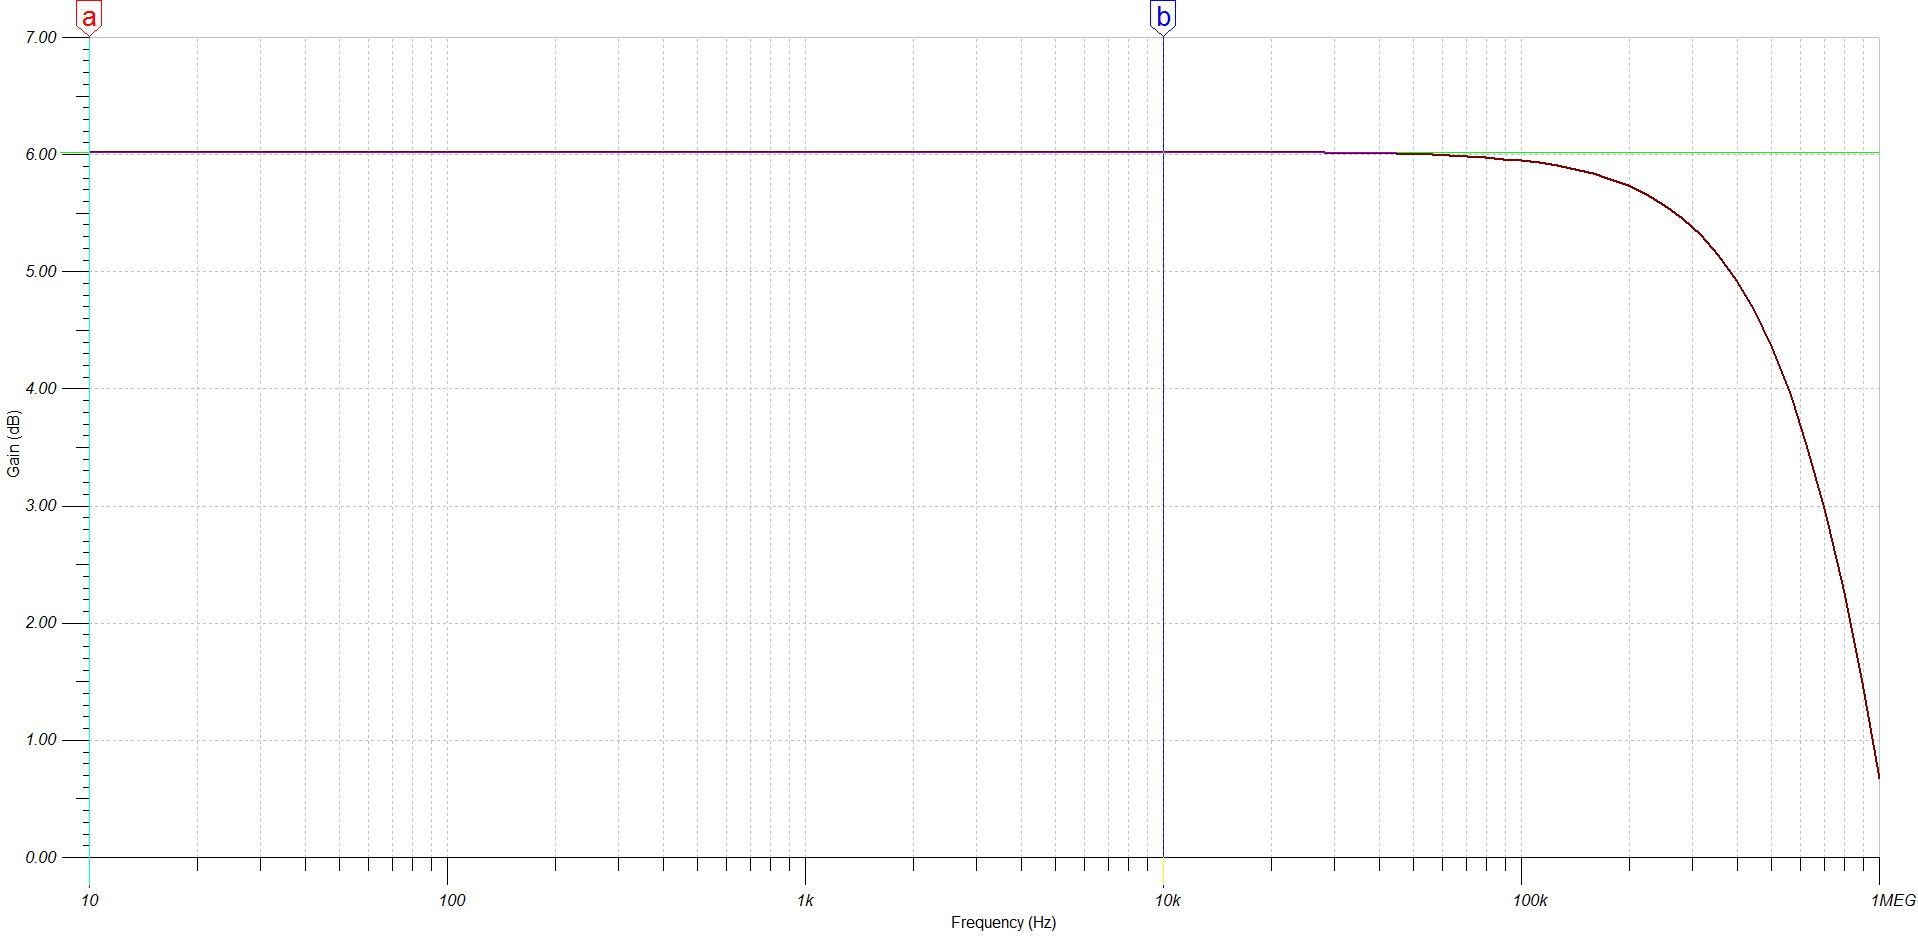
\includegraphics[width=\linewidth]{./res/gain.jpg}
	\caption{Γράφημα πρακτικού κέρδους}
\end{figure}
\begin{figure}[H]
	\centering
	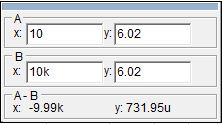
\includegraphics{./res/gaincalc.jpg}
	\caption{Υπολογισμός πρακτικού κέρδους}
\end{figure}

\subsection{Διαφορά φάσης}

Με βάση την παρακάτω μέτρηση, παρατηρούμε ότι η διαφορά φάσης είναι πολύ κοντά
στο \SI{0}{\degree}. Με άλλα λόγια, το σήμα εισόδου είναι σε φάση με το σήμα
εξόδου, το οποίο είναι λογικό, εφόσον το κύκλωμα είναι ένας μη-αναστρέφων
ενισχυτής.

\begin{figure}[H]
	\centering
	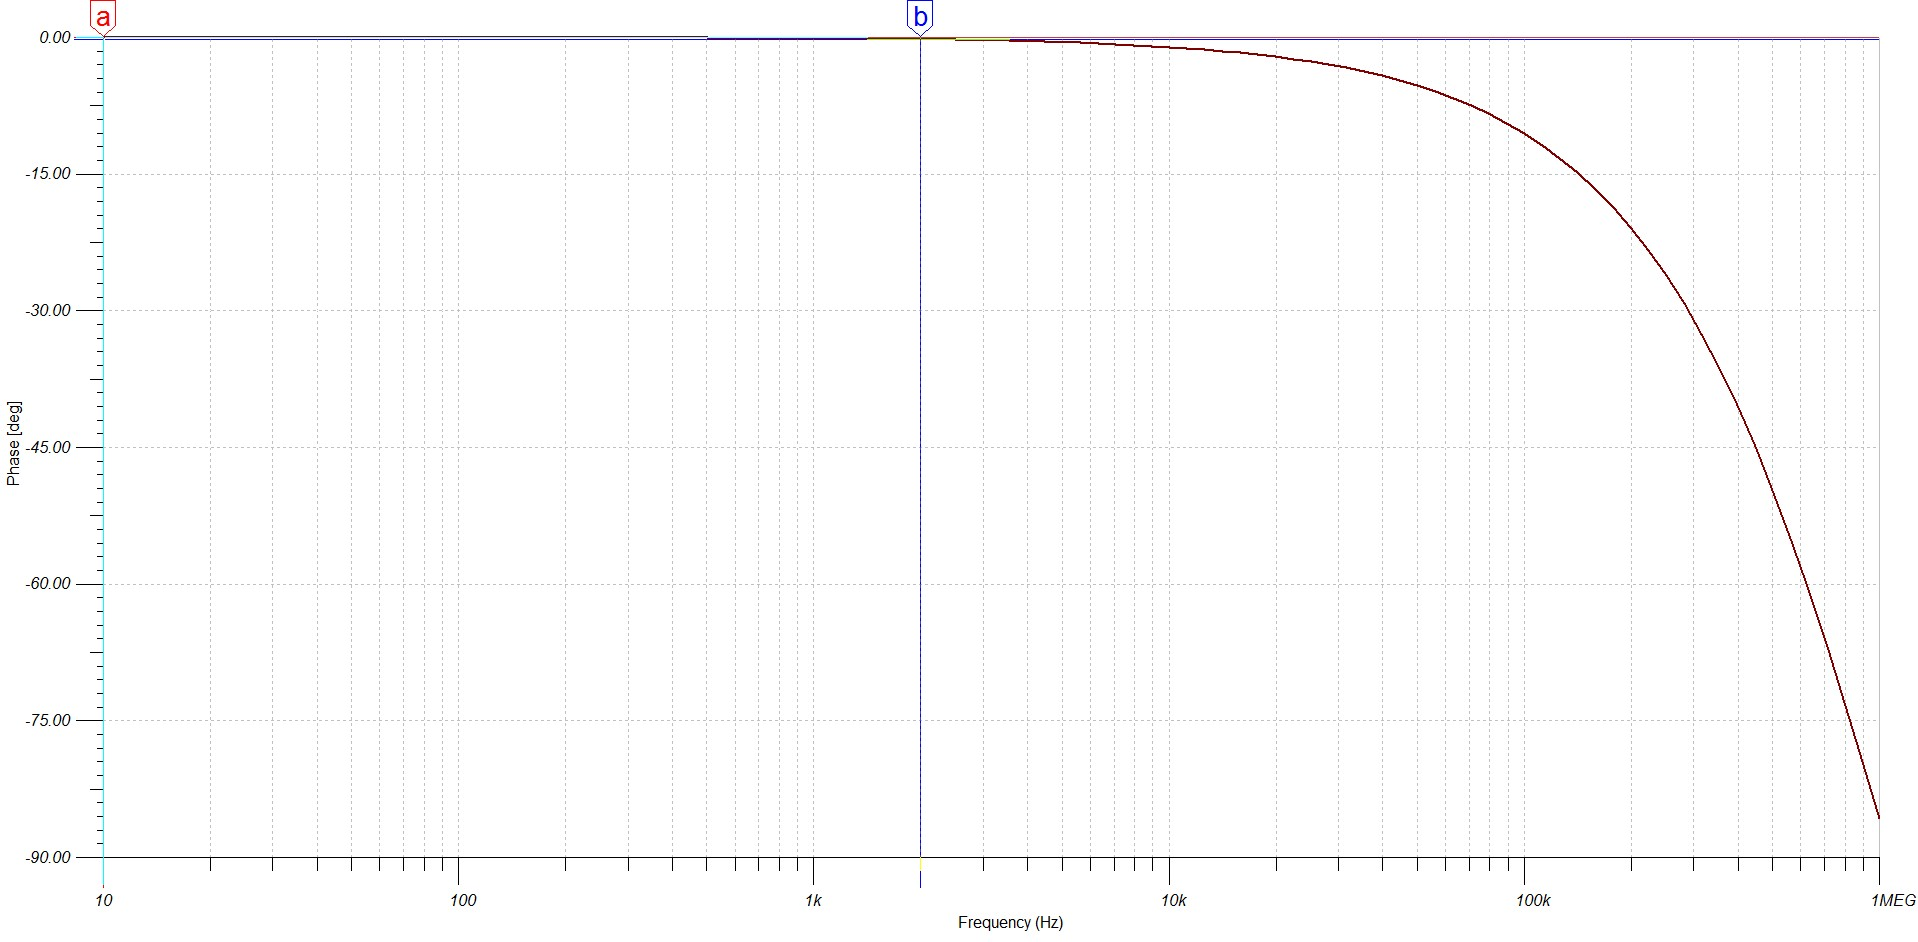
\includegraphics[width=\linewidth]{./res/phase.jpg}
	\caption{Γράφημα φάσης}
\end{figure}
\begin{figure}[H]
	\centering
	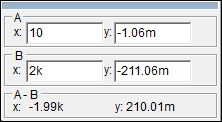
\includegraphics{./res/phasecalc.jpg}
	\caption{Υπολογισμός διαφοράς φάσης}
\end{figure}

\section{Αύξηση συχνότητας}

\begin{itemize}
	\item Διατηρώντας το πλάτος του σήματος εισόδου σταθερό αυξήστε την
		συχνότητα εισόδου σύμφωνα με τον παρακάτω πίνακα. Τι
		παρατηρείτε; Πού οφείλεται;
\end{itemize}

Παρατηρούμε ότι το κέρδος μένει ίδιο όσο και να αυξήσουμε την συχνότητα
εισόδου. Αυτό οφείλεται στο ότι για να αυξηθεί το κέρδος, πρέπει να αυξηθεί και
το πλάτος του σήματος.

\begin{center}
\begin{tabular}{|l|l|}
	\hline
	$F(\SI{}{\hertz})$ & $A(\SI{}{\decibel})$ \\
	\hline
	$\SI{1}{\kilo\hertz}$ & \SI{6.02}{\decibel} \\
	\hline
	$\SI{10}{\kilo\hertz}$ & \SI{6.02}{\decibel} \\
	\hline
	$\SI{50}{\kilo\hertz}$ & \SI{6.02}{\decibel} \\
	\hline
	$\SI{100}{\kilo\hertz}$ & \SI{6.02}{\decibel} \\
	\hline
	$\SI{500}{\kilo\hertz}$ & \SI{6.02}{\decibel} \\
	\hline
	$\SI{1}{\mega\hertz}$ & \SI{6.02}{\decibel} \\
	\hline
	$\SI{1.5}{\mega\hertz}$ & \SI{6.02}{\decibel} \\
	\hline
	$\SI{2}{\mega\hertz}$ & \SI{6.02}{\decibel} \\
	\hline
\end{tabular}
\end{center}

\section{Υλοποίηση σε breadboard}

\begin{itemize}
	\item Παρουσιάστε το κύκλωμά σας υλοποιημένο σε breadboard μέσω
		της εφαρμογής Tinkercad.
\end{itemize}

Για την συνδεσμολογία χρησιμοποιούμε το pinout του τελεστικού ενισχυτή ως reference:
\begin{figure}[H]
	\centering
	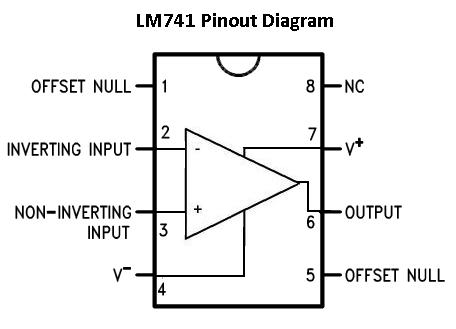
\includegraphics{./res/pinout.jpg}
\end{figure}

\begin{figure}[H]
	\centering
	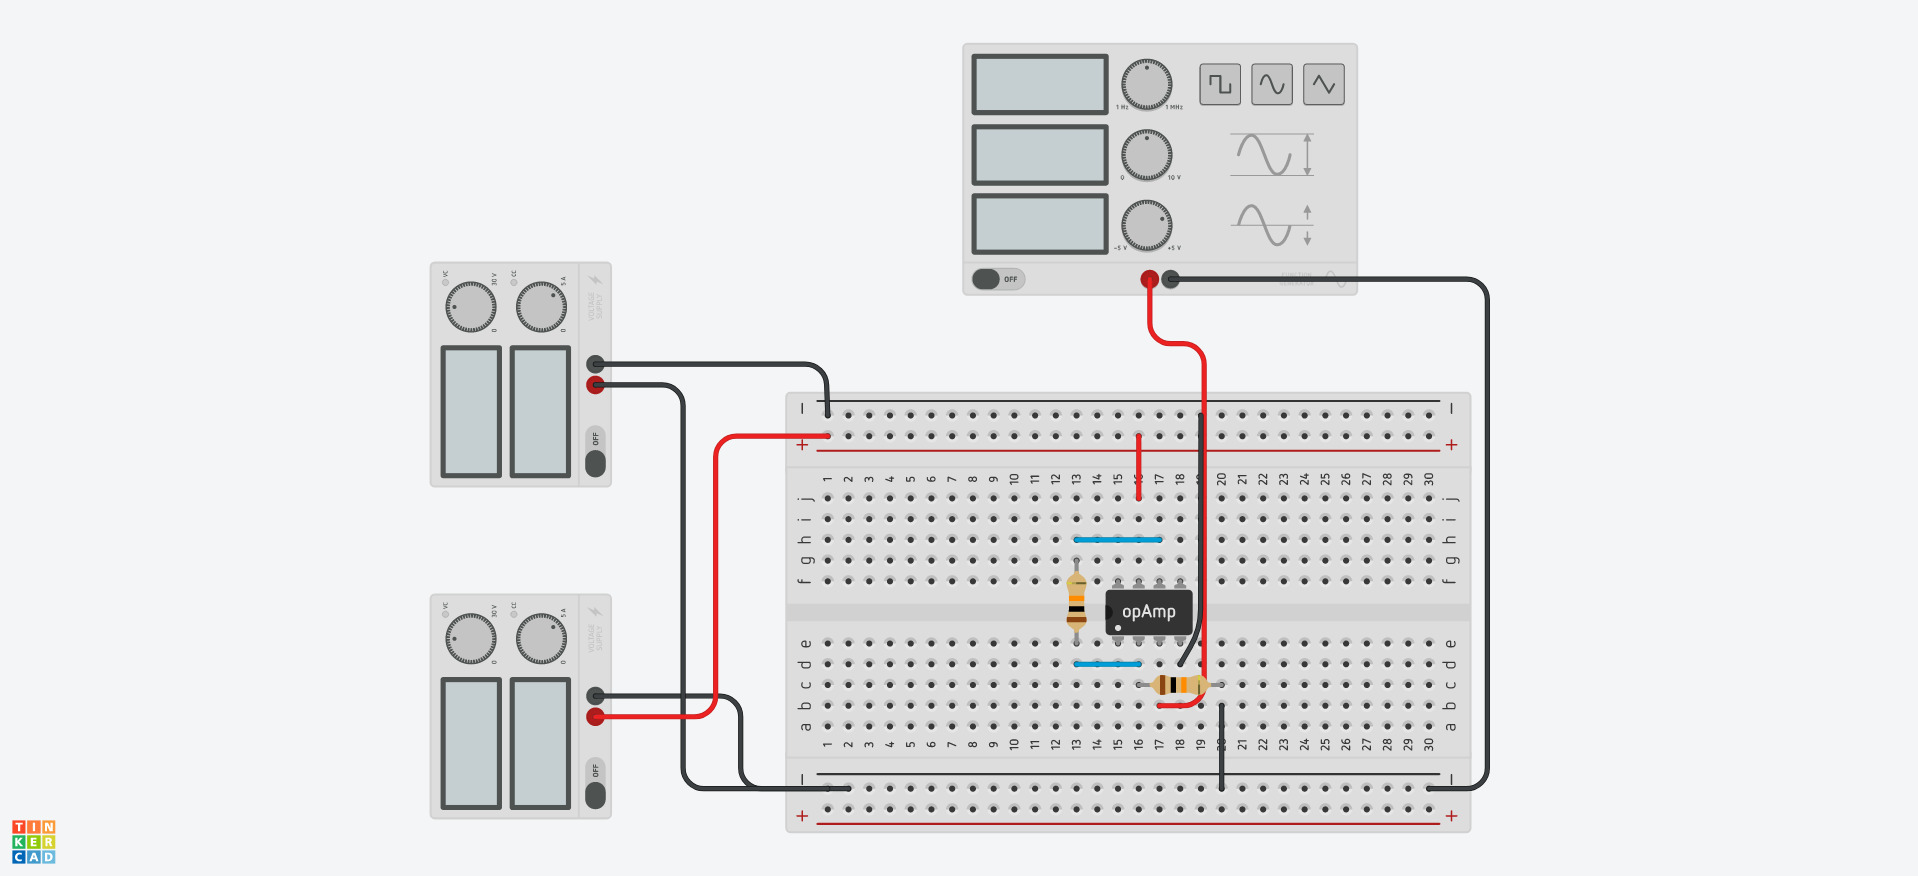
\includegraphics[width=\linewidth]{./res/bread.jpg}
\end{figure}

\end{document}
